% !TeX root = ../thuthesis-example.tex

\chapter{经典故障场景分析}\label{chap-failure-scenarios}

\section{单节点磁盘写满}

\subsection{故障检测方法}

目前IoTDB集群中有两种单节点磁盘写满的故障检测方式。

第一种是定期预防式的诊断,通过ConfigNode和DataNode的心跳完成。ConfigNode和DataNode交换的心跳包中会带有该DataNode节点的磁盘最大容量和目前的使用情况。如果目前的使用率已经超过了预先设置的阈值,那么ConfigNode就会将该节点标志为只读的状态。

第二种是发生时的临诊,通过DataNode在写入过程中的自检来完成。在DataNode服务某一个写入请求在文件系统上真正写入数据之前,会进行可写入性的检查,如果发现此时磁盘空间不足,那么本次写入请求就不会执行,并且返回给Session本次节点只读的状态。

\subsection{高可用容错方案}

\begin{figure}
    \centering
    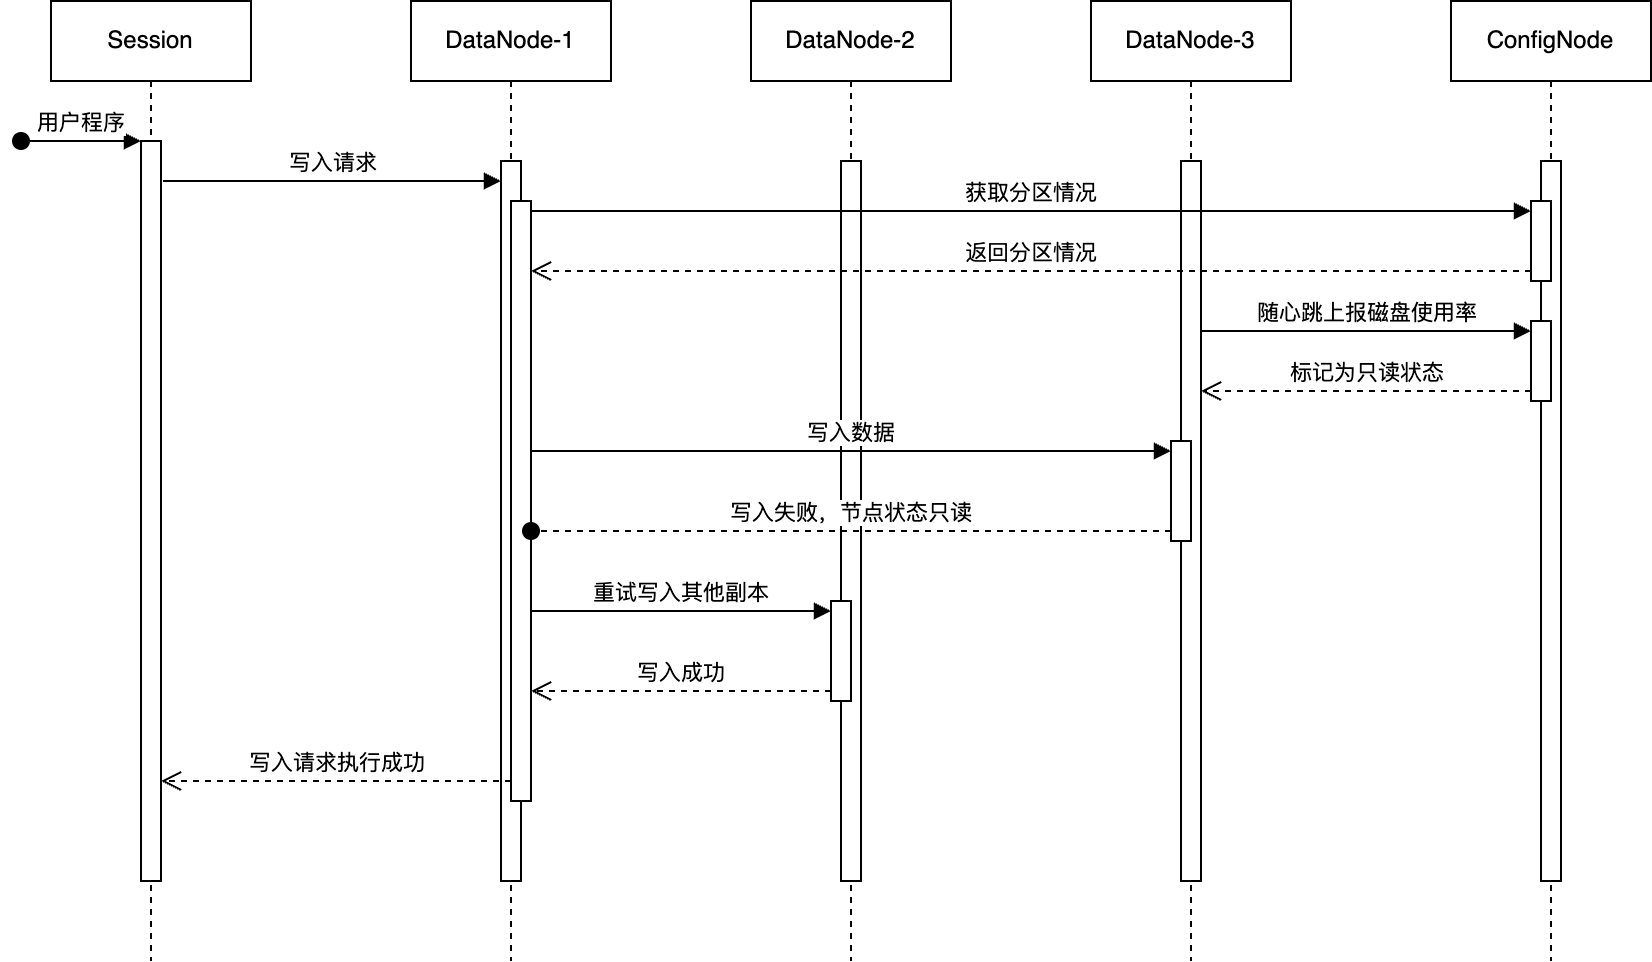
\includegraphics[width=0.99\linewidth]{c05-diskfull.png}
    \caption{单节点磁盘写满的高可用容错时序图}
    \label{fig:c05-diskfull}
  \end{figure}

图\ref{fig:c05-diskfull}给出了单节点磁盘写满的完整容错时序图。

可以看到,再某一个时刻,DataNode3的磁盘使用情况超过了阈值,并且在下一次和ConfigNode上报心跳的时候将这一情况上报给了ConfigNode。ConfigNode会将该节点标记为ReadOnly,并且在后台尝试将该节点上的所有Region的Leader转移给其他的副本,并且标记这些副本的状态为只读。

对于读请求来说,无论是故障发生时的在途请求,还是故障发生之后的新请求,都能够正常执行,不受任何影响。

对于写请求来说,则通过前一章节描述的故障错误转移的方式来实现容错。
对于故障发生之后的写入请求来说,在写入的规划阶段,规划器能够从ConfigNode这边拿到最新的分区情况,此时规划器会将本次的请求给路由到其他可以写入的副本上,从而避免错误的发生。
对于故障发生时就在执行的在途请求,则是通过Session和Coordinator侧的重试来保证数据的正确写入。以图中的写入请求为例,该请求在规划时DataNode3并没有标记为只读状态,因此规划的结果是将数据写入到DataNode3中。然而,在数据写入之前,DataNode3的状态变更为只读,无法再服务外部的写入请求。此时,写入到该节点的操作会返回只读的异常状态,DataNode1会在Coordinator侧捕捉这个错误异常,并且重试。重试时,Coordinator会选择其他的可用副本(在本示意图中为DataNode2),Coordinator会尝试将数据写入正常运行的DataNode2中,最终实现数据的成功写入。


\section{进程宕机}

\subsection{检测方法}
ConfigNode进程宕机和DataNode的进程宕机(kill -9, OOM)等场景下,可以通过ConfigNode Leader建立的心跳通道断开被直接发现。
具体来说,ConfigNode Leader和DataNode之间的心跳通道是基于Thrift构建的,底下的传输方式为Thrift的TSocket,在具体实现中,TSocket是基于TCP实现的。当一个进程突然崩溃或被强制终止时,操作系统会立即关闭该进程打开的所有TCP连接,因此ConfigNode Leader的Thrift连接能够捕获这些TCP层面的信号,立即得知连接已断开,并向应用程序报告。即使TCP连接没有立即断开,如果对端进程已经停止响应,任何尝试通过该连接进行读写操作都会导致I/O异常。Thrift框架能够捕获这些I/O异常,例如连接超时、连接拒绝等,从而判断对端进程已失效。

\subsection{高可用容错方案}

对于进程宕机的情况,由于DataNode同时要处理来自客户端Session的连接,又需要应对集群内部的Coordinator转发的请求,因此高可用方案需要同时满足这两个场景的可用。

\begin{figure}
    \centering
    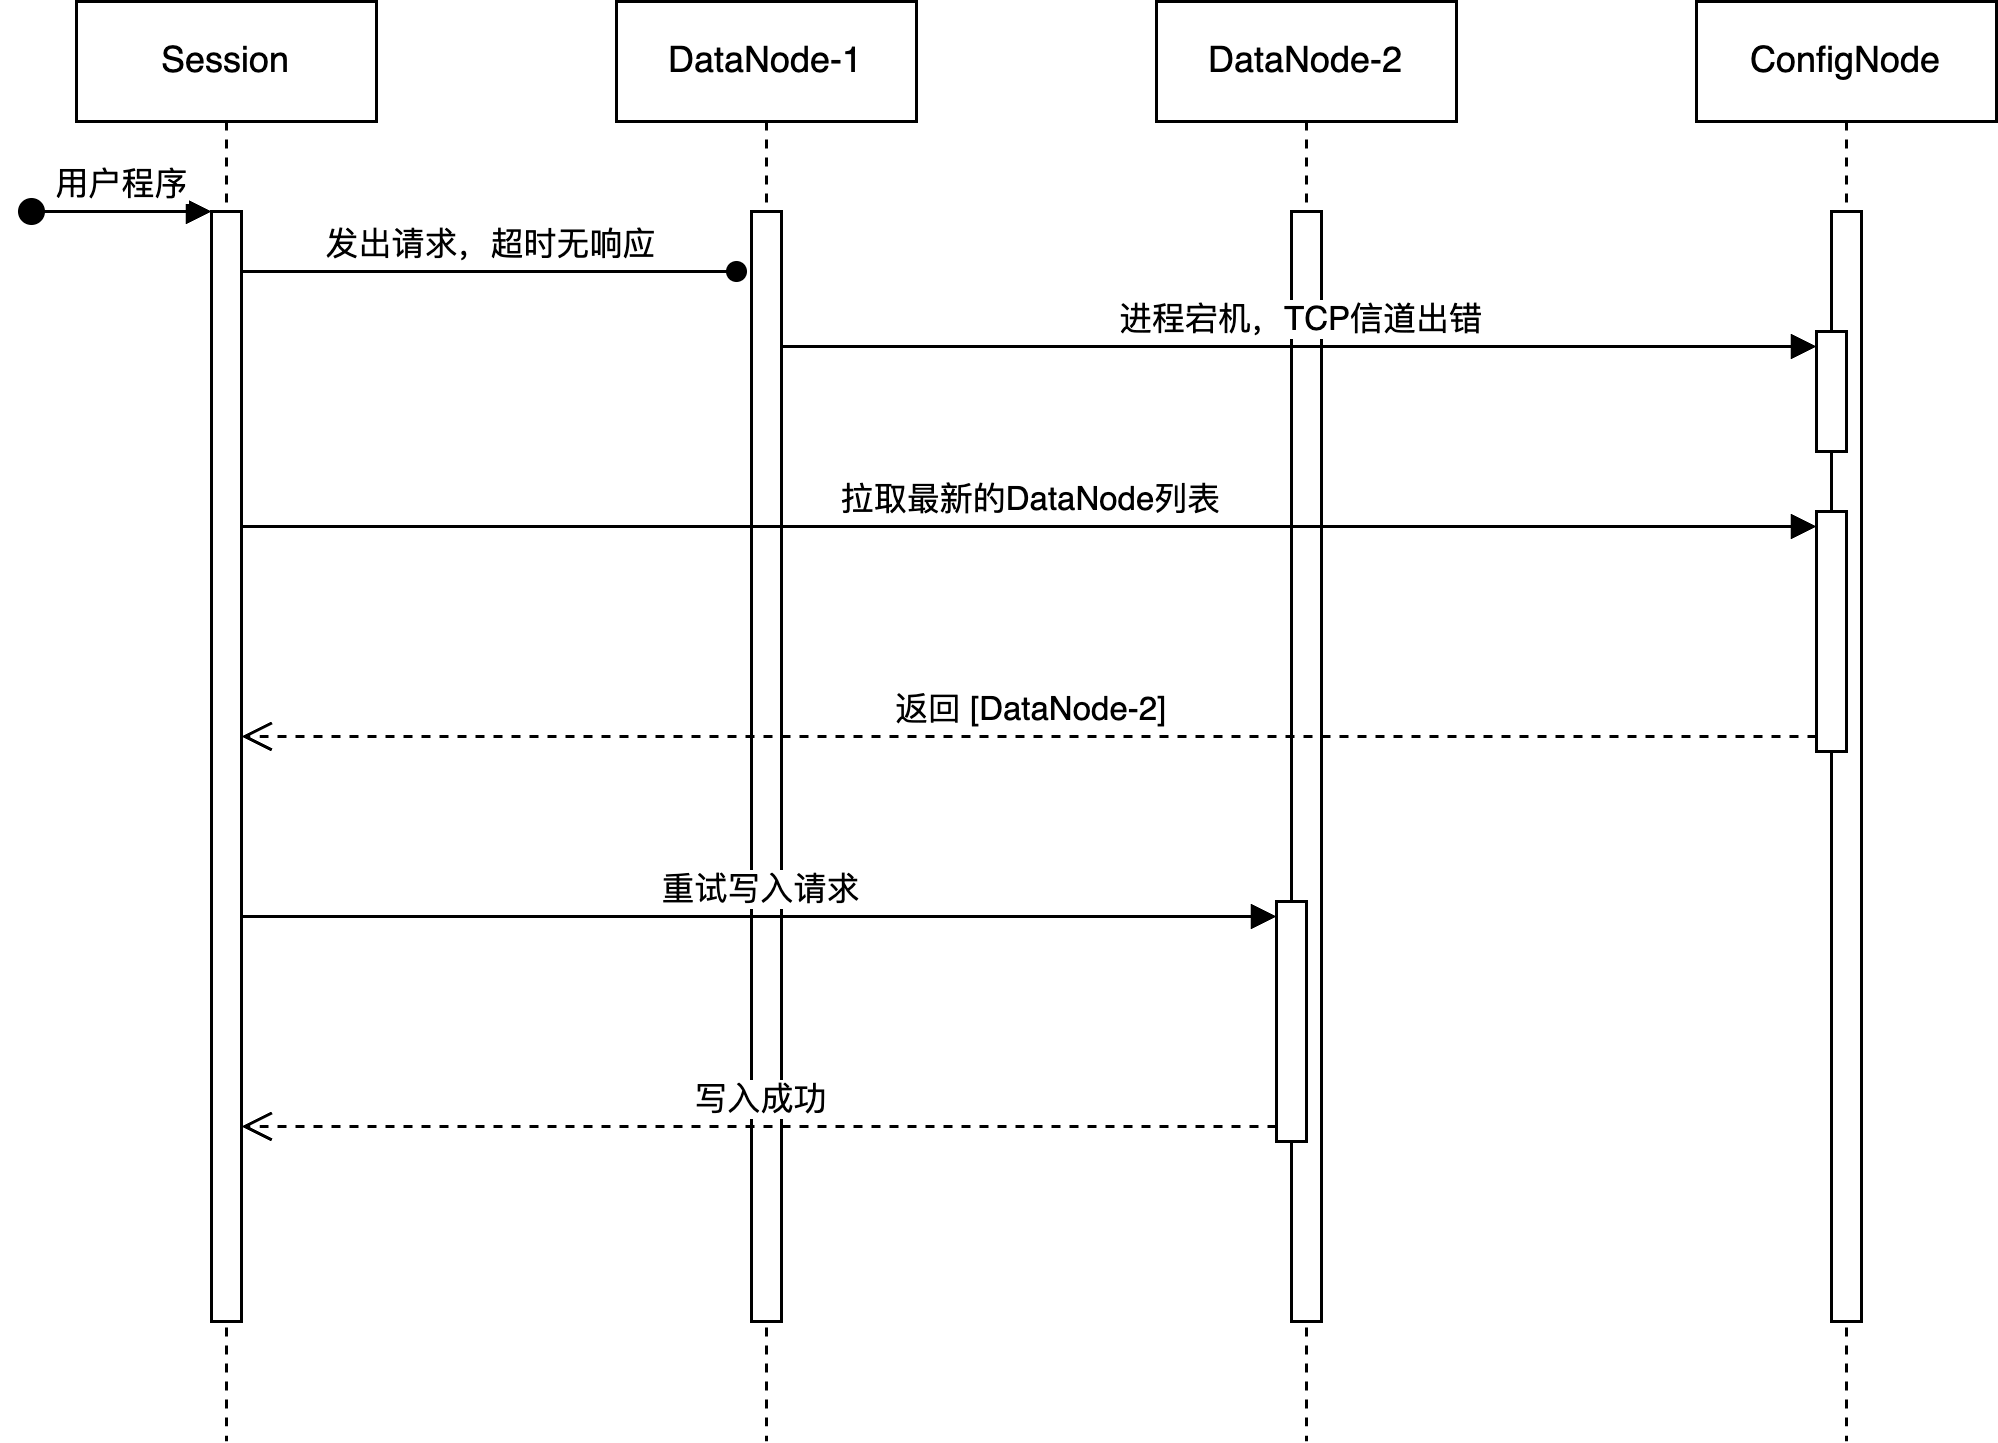
\includegraphics[width=0.99\linewidth]{c05-process-down-1.png}
    \caption{单节点进程宕机的高可用容错时序图}
    \label{fig:c05-process-down-1}
\end{figure}

图\ref{fig:c05-process-down-1}展示了高可用容错方案对于因DataNode宕机导致的用户连接直接失效的解决方案。图中DataNode1在处理Session的请求的时候出现了宕机,会导致Session的该请求超时无响应。
DataNode1宕机之后,ConfigNode可以通过心跳的方式检测出DataNode1的异常,并且更新该节点的状态。后续,由于Session具备后台进程会持续地从ConfigNode拉取最新的DataNode列表,因此最新一次的拉取将给出只有DataNode2存活的事实。
此时,Session会尝试重新向DataNode2发送请求。由于此时DataNode2正常工作,因此本次请求能够被正常处理,从而使用户的请求最终能够正常写入。


对于别的Coordinator连接到该DataNode上的请求,则会通过跟\ref{fig:c05-diskfull}相同的流程图来对其他的数据副本进行重试。

\section{对称网络分区}

\subsection{检测方法}
当DataNode节点和其他的节点出现了对称网络分区的情况下,由于节点依旧存活,所以不会因为关闭TCP信道的原因被发现。
此时,则需要通过上述的Phi Accural算法对节点的网络分区进行识别。具体来说,由于发给该节点的心跳都没有反应,在超过一定的时间之后,Phi Accrual算法就会判断该节点不可达,从而依然将节点的状态设置成UNKNWON

\subsection{高可用容错方案}

对于因为网络分区而失败的请求,则会通过跟\ref{fig:c05-diskfull}相同的流程图来对其他的数据副本进行重试。

\section{非对称网络分区}

\subsection{检测方法}
当DataNode节点和其他的DataNode节点出现了非对称网络分区的情况下,由于和ConfigNode之间的心跳通道能够正常交换心跳包,因此不会被ConfigNode的心跳机制所检测到。此时,则需要通过前文描述的拓扑感知的方式来进行判断。ConfigNode Leader会要求所有的DataNode定期测试和其他的所有DataNode的内部服务端口的连通性,并且上报每次的连通性的测试结果。
ConfigNode使用Phi Accural的检测算法对联通心跳进行检测,并实时判断。

\subsection{高可用容错方案}

\begin{figure}
    \centering
    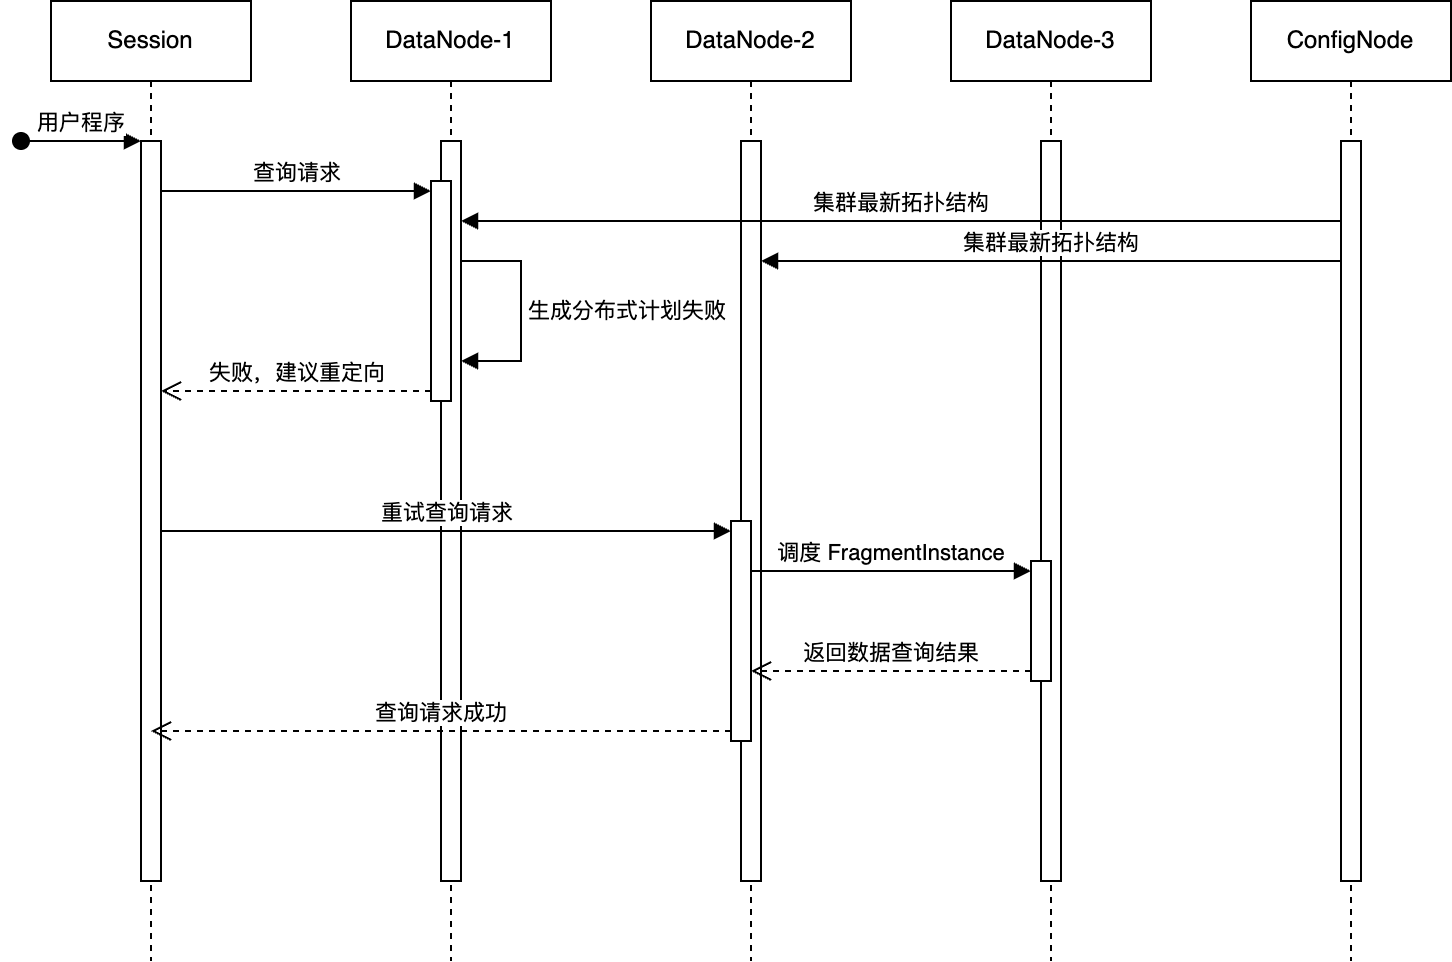
\includegraphics[width=0.99\linewidth]{c05-partition-asym.png}
    \caption{非对称网络分区的高可用容错时序图}
    \label{fig:c05-partition-asym}
\end{figure}

在非对称网络分区的情况下,需要Session和Coordinator两侧的协同才能解决这一类的问题。

图\ref{fig:c05-partition-asym}给出了非对称网络分区的高可用容错时序图。假设集群DataNode1和DataNode3之间出现了非对称网络分区。客户端连接到了DataNode-1上,并发送了查询请求。DataNode1在解析了查询请求之后,根据ConfigNode下发的最新集群拓扑,发现root fragment instance必须调度到DataNode3上,但是由于非对称网络分区的存在,该调度无法实现,因此DataNode1会返回失败的状态码,并附带重定向该请求的建议。

Session侧在获得重定向的失败消息之后,会尝试将该请求重定向到DataNode2上执行。由于DataNode2并不存在网络分区,能够和集群内的所有节点连接,因此查询规划能够顺利生成和调度,在多个DataNode之间进行数据的实际查询,完成本次的查询请求,将结果返回给Session的客户。

\section{ConfigNode节点脑裂}

ConfigNode是集群的大脑,负责管理集群的节点基础信息、现在的状态、集群的拓扑网络结构、集群的分区信息等,并且ConfigNode上运行着诸多后台的服务,包括负载均衡、Region迁移等服务。
我们需要保证ConfigNode服务的高可用,因此我们会运行多个ConfigNode的副本,每一个副本都保持了相同的数据,但是同一时刻只能有一个主副本发号施令,决定服务的实际状态。当主副本所在的ConfigNode节点出现宕机的时候,其他的副本则会通过选举流程产生一个新的主副本,接替相关的任务。

这种机制可能会出现脑裂的情况。具体来说,如果主副本短暂地发生了网络分区的情况,其他副本如果此时发起选举并且被正式选举为主副本,此时旧的主副本的网络分区恢复,且旧的主副本还没有意识到自己已经不再是Leader的情况下,就会导致集群中有两个主副本同时发号施令,从而出现所谓的脑裂情况。


我们通过设置Leader Lease和选举最小超时时间的方式来避免脑裂的结果。具体来说,如果Leader在一段时间没有收到来自大多数节点的心跳,那么Leader此时就会自己主动结束Leader的身份。而新的节点的最小选举超时需要大于Lease的时间。

这样做的好处在于能够保证集群的脑裂情况不会出现,但是坏处在于集群可能有一小段的时间ConfigNode的服务无法提供。此时,Session和Coordinator上请求ConfigNode节点的服务需要进行等待重试,防止出现这样的情况。

\begin{figure}
    \centering
    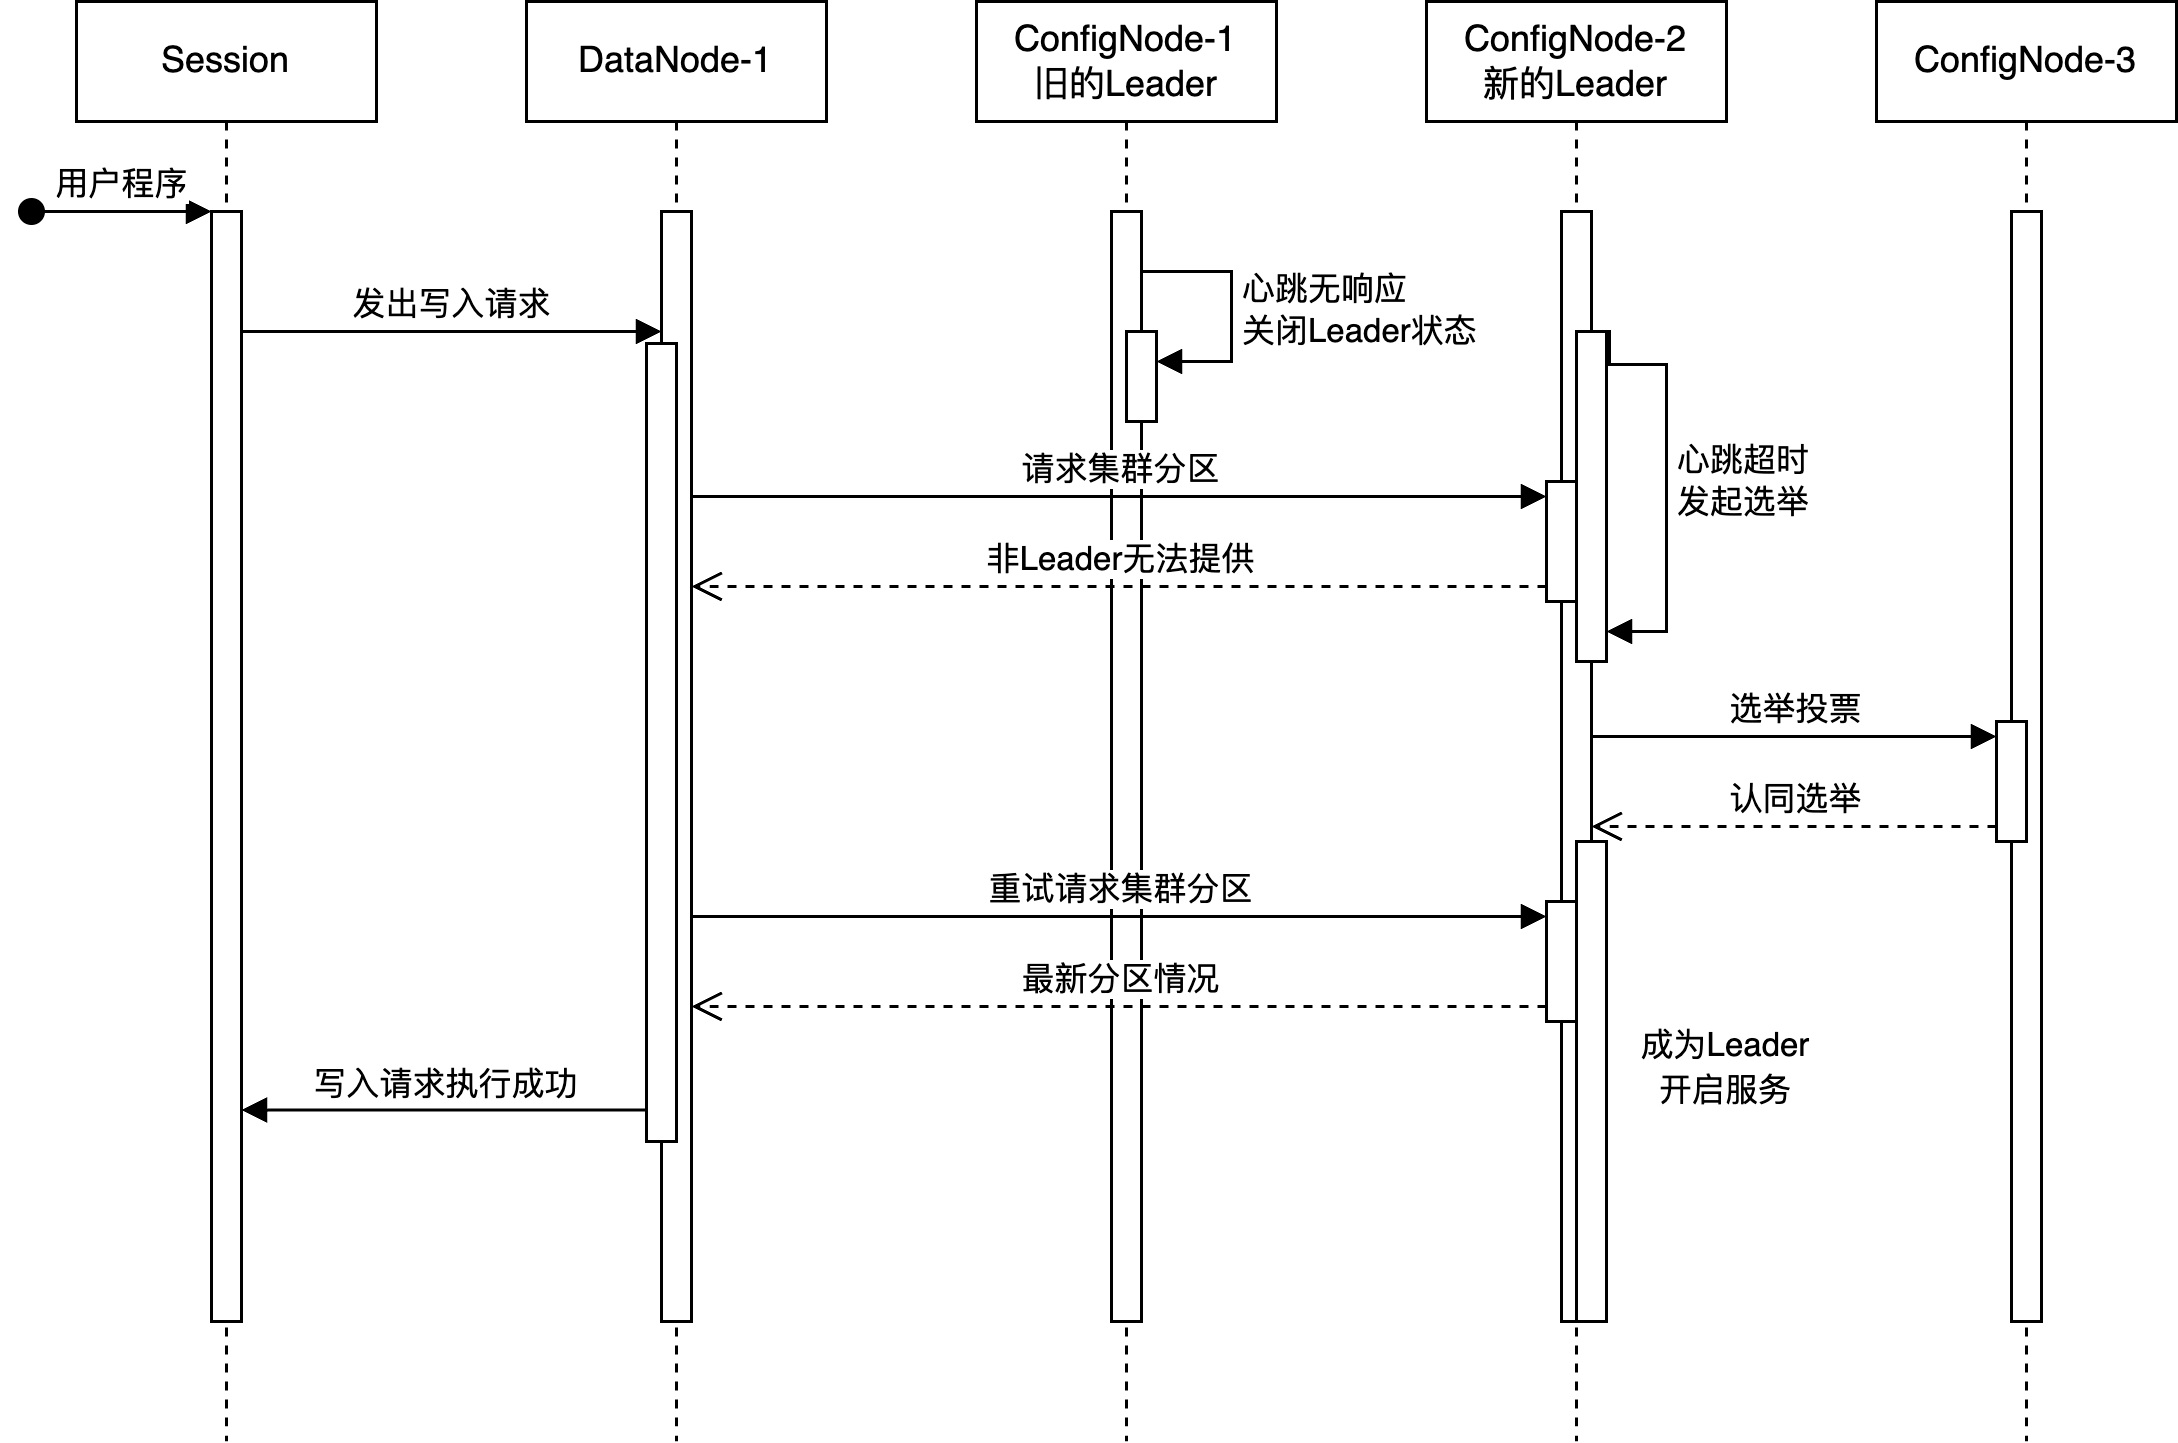
\includegraphics[width=0.99\linewidth]{c05-brain-split.png}
    \caption{ConfigNode服务的高可用容错时序图}
    \label{fig:c05-brain-split}
\end{figure}

图\ref{fig:c05-brain-split}展现了ConfigNode因为短暂的网络分区而导致服务不可用的情况下的高可用时序图。其中,ConfigNode-1是旧的Leader,由于和剩下的两个副本ConfigNode-2/ConfigNode-3之间出现了网络分区,导致在一段时间心跳无响应的状态下主动结束了Leader的服务。此时集群中没有ConfigNode节点能够提供服务。

此时,如果用户的写入和查询请求需要向ConfigNode获取分区等服务,那么这些请求就不能得到响应。此时,DataNode2需要等待一段时间,再进行重试。

在等待的这段时间里,ConfigNode-2率先出现选举超时,开始新一轮的选举,并在ConfigNode3的支持下成功当选最新一期的Leader,并正常开启了ConfigNode 的服务。此时,DataNode2再重试请求分区,ConfigNode2能够正常对其提供服务,DataNode也能够顺利完成请求的执行。

\section{集群变更状态下的一致性}

\subsection{错误检测}

在分布式IoTDB中,集群变更操作如Region迁移、节点扩缩容是保持集群拓展能力、负载均衡能力的必要手段。然而,这些操作在执行过程中不可避免地会引入短暂的数据不一致性,这种一致性可能会导致用户数据写入失败。

严格来讲,这种短暂的不一致性并非系统设计上的错误,也并非在系统运行中出现的故障,而是系统在追求极致可用性目标时所做出的权衡。

根据CAP原理\cite{fox1999harvest},在一个分布式系统中,一致性(Consistency)和可用性(Availability)往往难以同时保证。具体而言,如果系统在集群变更期间必须严格维护数据的绝对一致性,则必须暂停所有用户的写入操作,直至变更完成。这种做法虽然能够确保数据的一致性,但却极大地牺牲了系统的可用性,导致用户在一段时间内无法正常访问或操作数据。

IoTDB在设计的时候,选择在保证最终一致性的前提下,允许短暂的数据不一致性。因此,用户的请求可以随时到达,即使集群正处在变更的过程中,也会通过上述所言的三级重试来最大化地满足用户的请求。

\subsection{高可用容错方案}

\begin{figure}
    \centering
    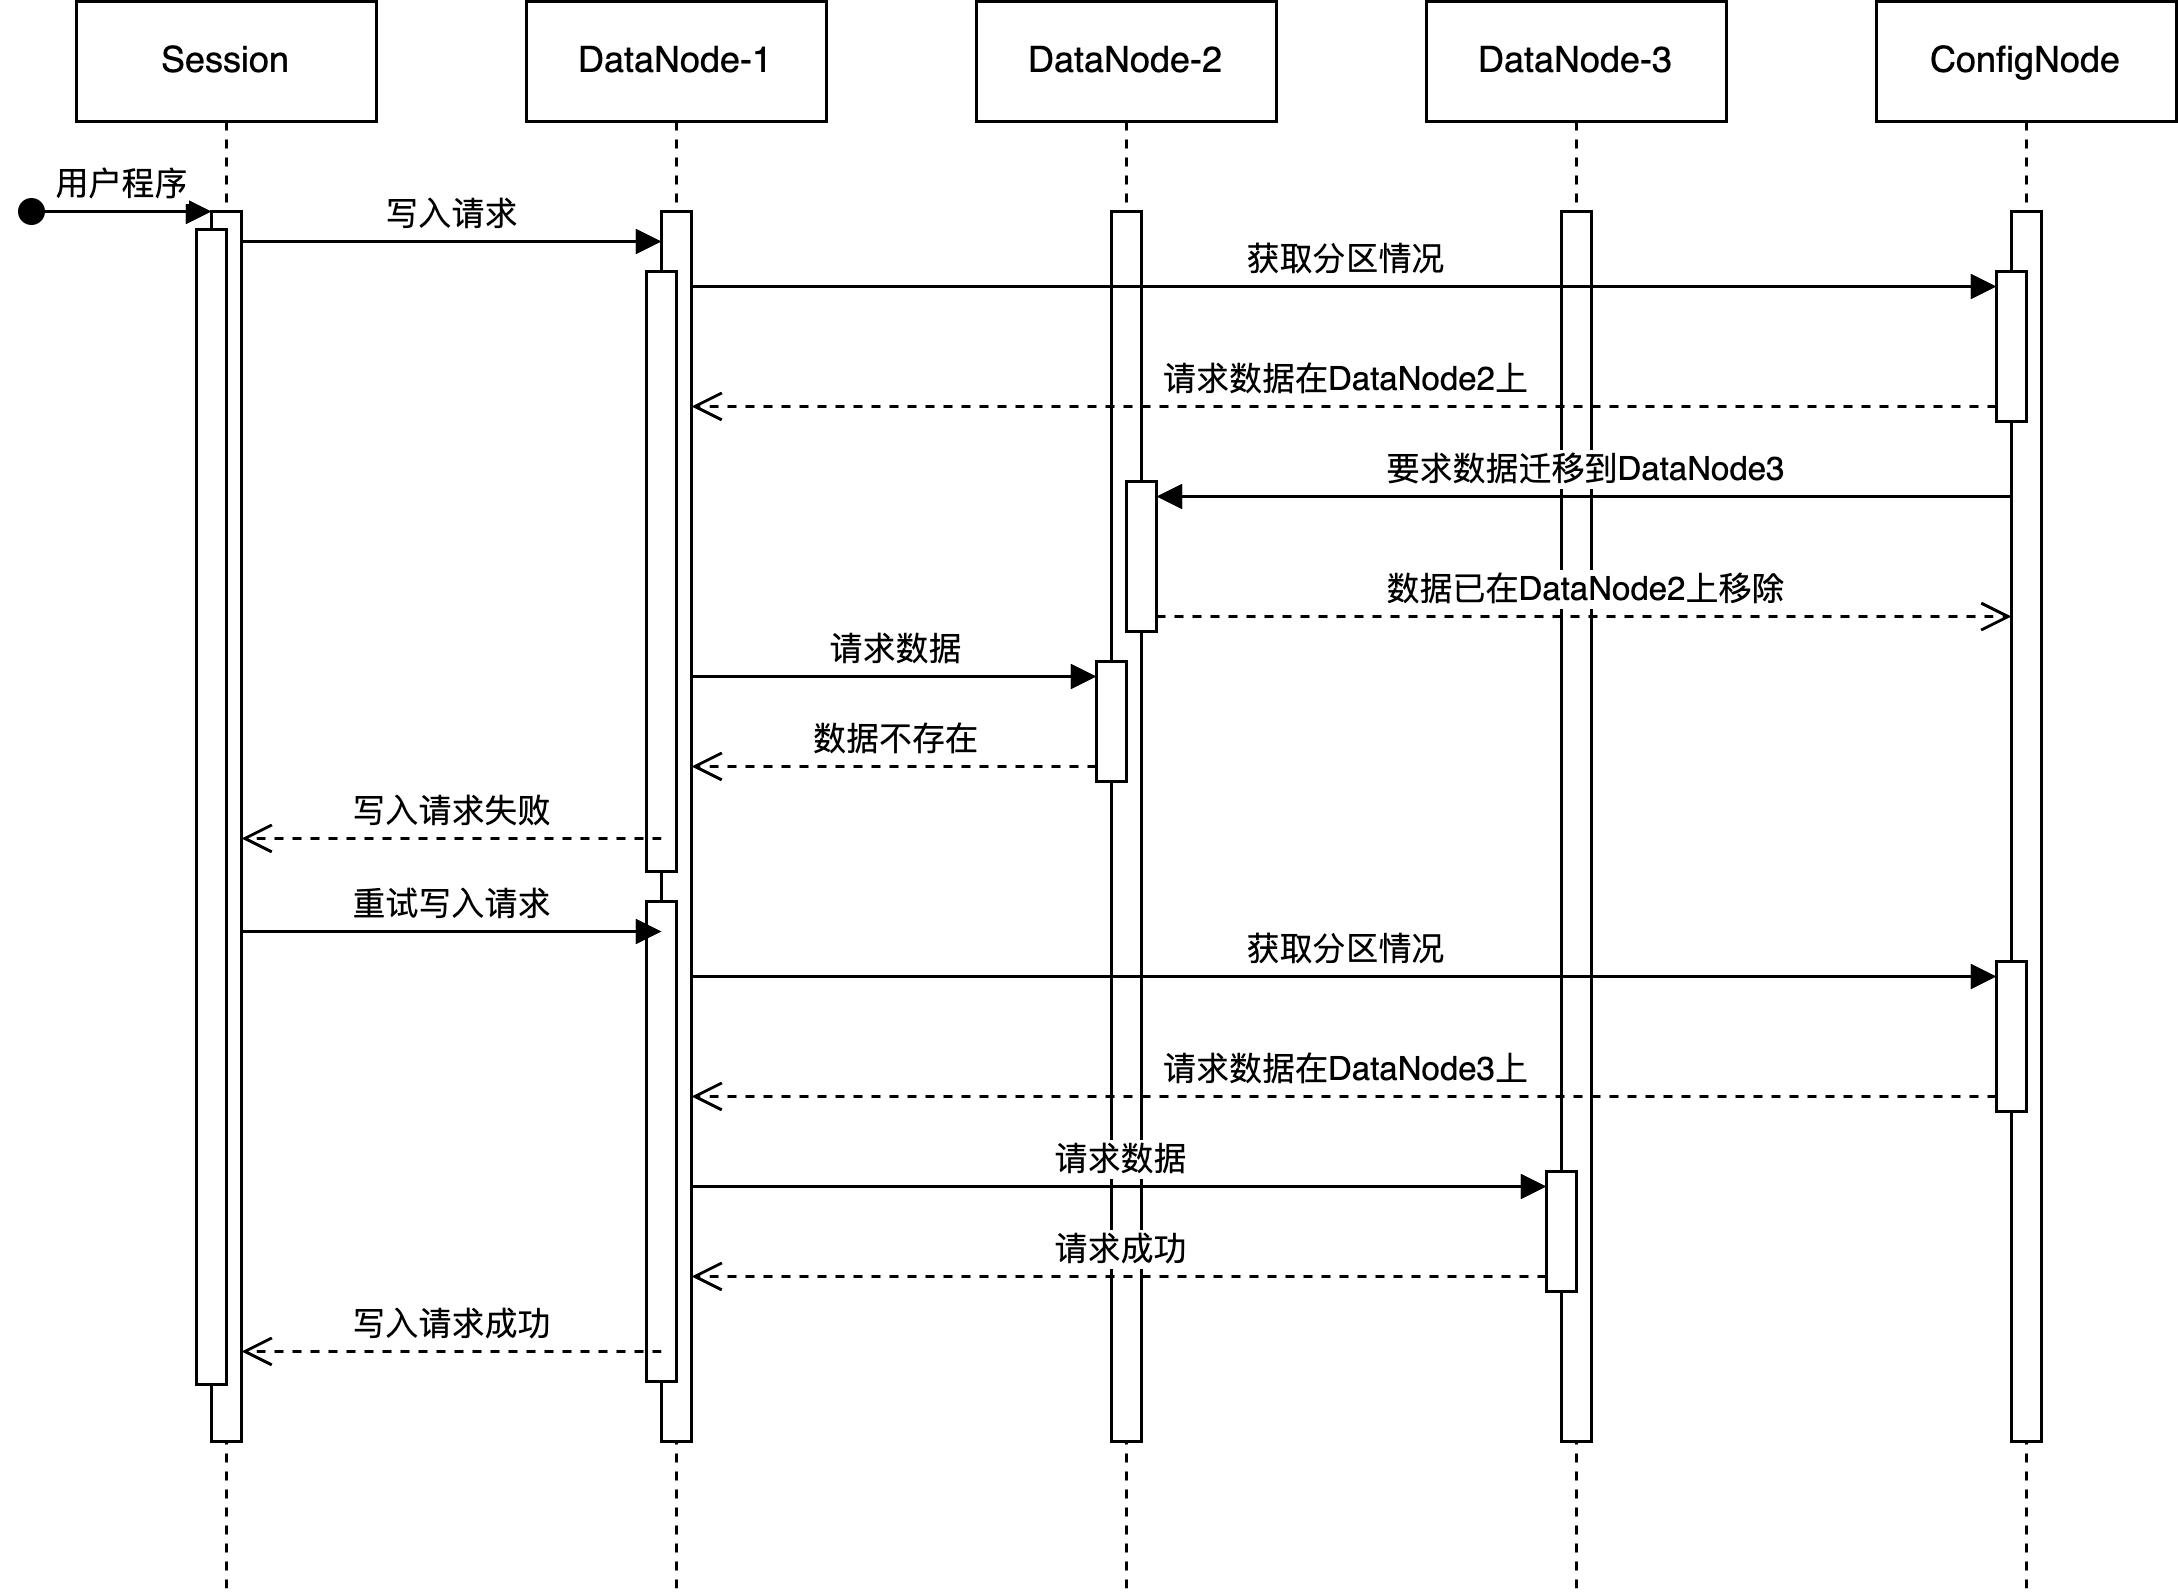
\includegraphics[width=0.99\linewidth]{c05-cluster-change.png}
    \caption{集群变更状态下高可用容错时序图}
    \label{fig:c05-cluster-change}
\end{figure}

图\ref{fig:c05-cluster-change}展示了在集群变更状态下系统的高可用容错时序图。用户在通过Session进行写入请求的时候,DataNode1先从ConfigNode这里获取了分区情况,并根据这个分区情况进行写入规划。然而,在规划期间,出于负载均衡的考虑,ConfigNode决定进行Region迁移的操作,将原本在DataNode2上的数据分区给迁移到DataNode3上。
写入规划对这一次Region迁移并不知情,并且继续向DataNode2发出请求,此时由于数据已被迁移出该节点,所以这个请求会以数据不存在的原因失败。
DataNode1会将这个情况返回给Session,并且附上重试的建议。Session会继续重试写入这个请求,这个请求会再次被发送到DataNode1上。此时,DataNode1会再次从ConfigNode这边获取最新的分区情况。此时最新的分区已经能够反映上次迁移的改变,因此DataNode1能够正确认识到数据此时存活在DataNode3上,从而向DataNode3发起请求,最终成功获取数据,本次写入也能顺利执行。